\chapter{Architecture Synthesis}
\label{chap:arch-syn}
This chapter focuses on the architecture synthesis, i.e. synthesising a fault-tolerant architecture. It takes the initial architecture (as a netlist) to be made fault-tolerant, a component library, an application model and fault model as an input and synthesises a fault-tolerant architecture. The chapter will state the formal problem formulation. Furthermore it will present the solution strategy.


\section{Problem Formulation}
\label{sec:prob-for}
The problem can be formulated as follows: Given a netlist (components and their interconnections), a component library $\mathcal{L}$, an application graph $\mathcal{G}(\mathcal{O}, \mathcal{E})$ with a deadline $d_\mathcal{G}$ and a fault model $\mathcal{Z} = (\mathcal{VF}, \mathcal{CF}, v, c)$, determine a fault tolerant netlist such that the biochip is fault tolerant and it minimises the cost of the architecture.

The architecture provided by the designer is assumed to be an architecture that the designer knows well. By virtue of this the designer can specify exact faults that are perhaps typical faults or critical faults in the architecture. The inputs are modeled as described in \autoref{chap:sys}.
%In this thesis each netlist has a pre-defined average connection time, i.e. each connection in the netlist takes a pre-defined average time to traverse. The exact times are known once the physical routing is done though we do not have that yet.

\begin{figure}[H]
\centering
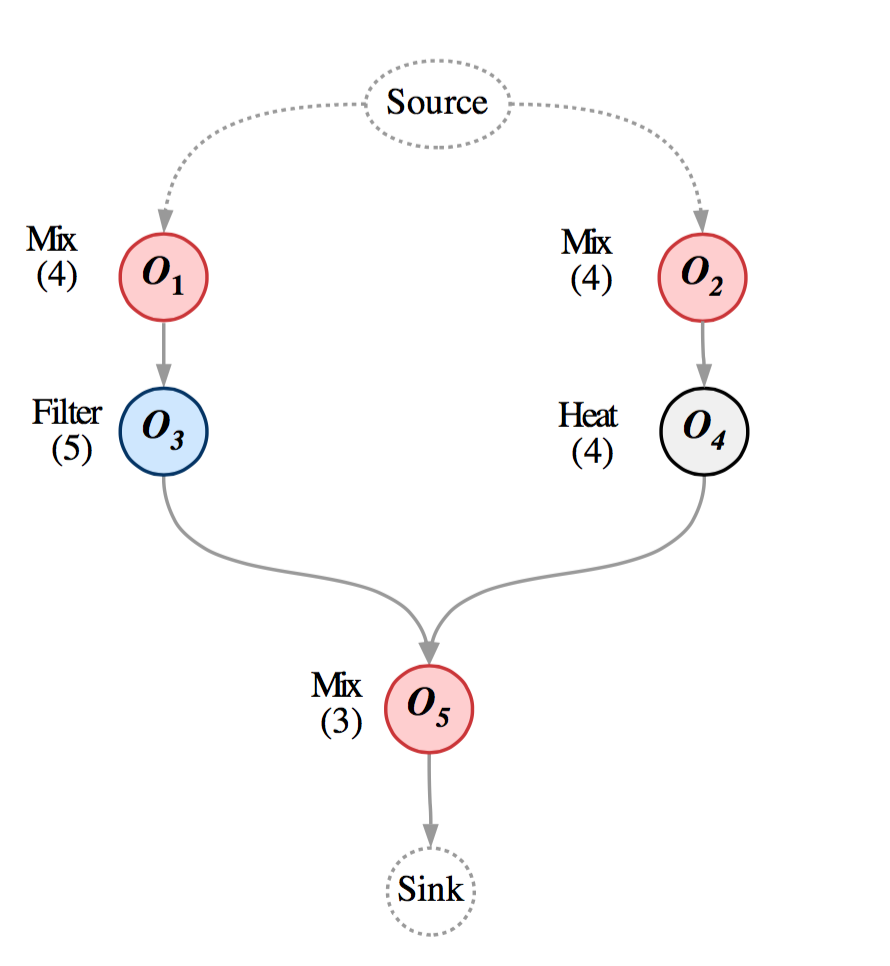
\includegraphics[scale=0.3]{figures/application-model.png}
\caption[Example application graph $\mathcal{G}$ for architecture synthesis]{Example application graph $\mathcal{G}$ for architecture synthesis}
\label{fig:arch-syn-application}
\end{figure}

\begin{figure}[H]
\centering
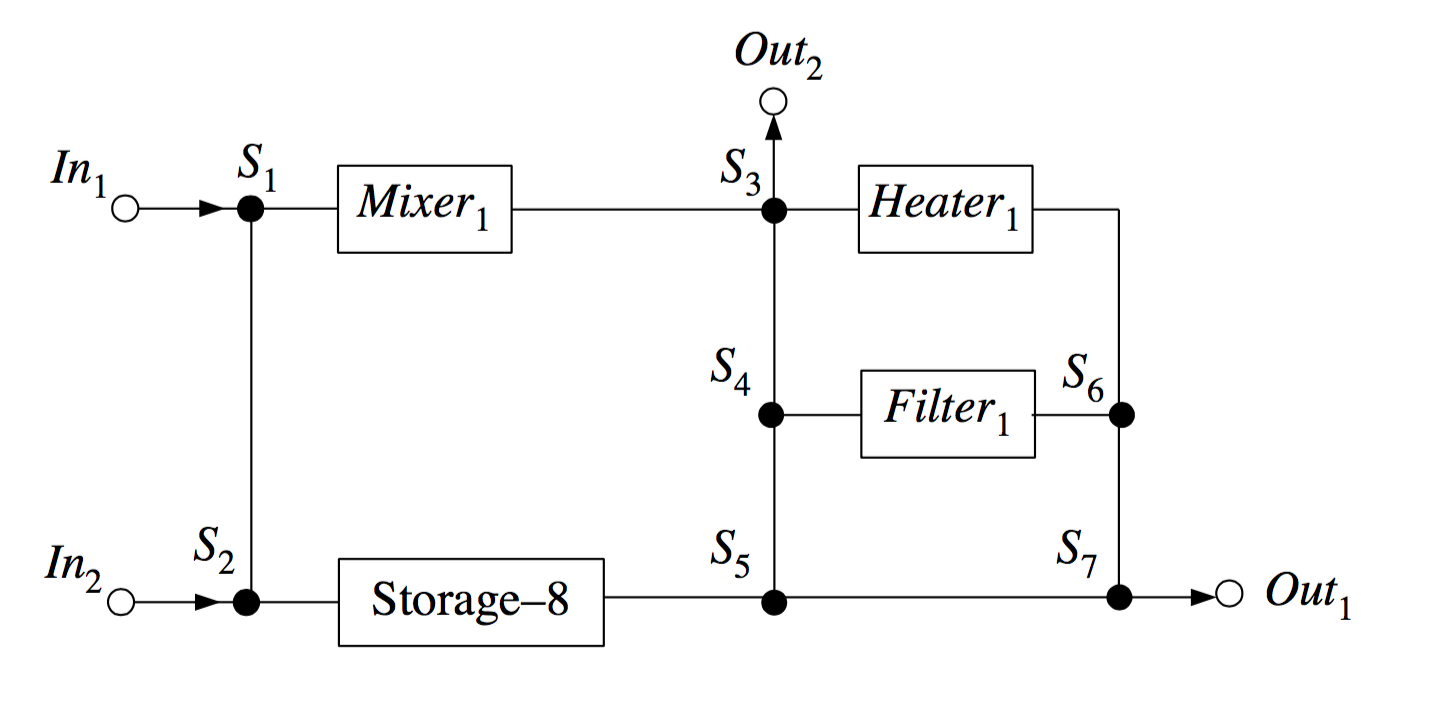
\includegraphics[scale=0.3]{figures/architecture.png}
\caption[Example architecture for architecture synthesis]{Example architecture for architecture synthesis}
\label{fig:arch-syn-arch}
\end{figure}

\begin{table}[H]
\centering
\caption{Example set of valve faults $\mathcal{VF}$ for architecture synthesis}
\begin{tabular}{| c | c | c | c |}
\hline
\textbf{Name} & \textbf{Vertex} ($N \in \mathcal{N})$ & \textbf{Valve affected} $(w)$ & \textbf{Type} $(t)$ \\ \hline
$VF_1$ & $Mixer_1$ & $v_5$ & Open \\ \hline
$VF_2$ & $S_6$ & $v_3$ & Open \\ \hline
$VF_3$ & $S_5$ & $v_2$ & Open \\ \hline
$VF_4$ & $S_3$ & $v_3$ & Open \\ \hline
\end{tabular}
\label{tab:arch-valve-faults}
\end{table}

\begin{table}[H]
\centering
\caption{Example set of channel faults $\mathcal{CF}$ for architecture synthesis}
\begin{tabular}{| c | c | c | c |}
\hline
\textbf{Name} & \textbf{Component} ($M \in \mathcal{N}, \notin \mathcal{S})$ \textbf{/ Connection} $D_{i, j} \in \mathcal{D}$ & \textbf{Type} $(t)$ \\ \hline
$CF_1$ & $Heater_1$ & Block \\ \hline
$CF_2$ & $Filter_1$ & Block \\ \hline
$CF_3$ & $S_2 \rightarrow$ Storage-8 & Block \\ \hline
$CF_4$ & $S_1 \rightarrow Mixer_1$ & Block \\ \hline
\end{tabular}
\label{tab:arch-channel-faults}
\end{table}

Considering the application graph $\mathcal{G}$ in \autoref{fig:arch-syn-application} and the architecture $\mathcal{A}$ in \autoref{fig:arch-syn-arch} we are interested in synthesising an architecture such that is tolerant to the faults given in \autoref{tab:arch-valve-faults} and \autoref{tab:arch-channel-faults} and that the cost of the architecture is minimised.\\
\autoref{fig:motivational-solution}a shows a straightforward solution to this problem, whereas \autoref{fig:motivational-solution}b shows an optimised solution to this problem. In the straightforward solution, which we assume that the designer could create without the help of our tool, a redundant component is added for each component that would be unable to perform its operation considering the fault model which thereby implies that the application graph in \autoref{fig:arch-syn-application} cannot complete. Fault-tolerant switches, $S_3, S_5$ and $S_6$, have been added to compensate for the failing valves. Similarly a redundant channel has been added to compensate for the blocked channel $S_2 \rightarrow$ Storage-8. No channel has been added to make the $S_1 \rightarrow Mixer_1$ channel redundant as it is not needed by virtue of $Mixer_2$. The cost of the architecture in \autoref{fig:motivational-solution}a is calculated to be 129. The calculation is the sum of the total number of valves and the total number of channels.

\begin{figure}
\centering
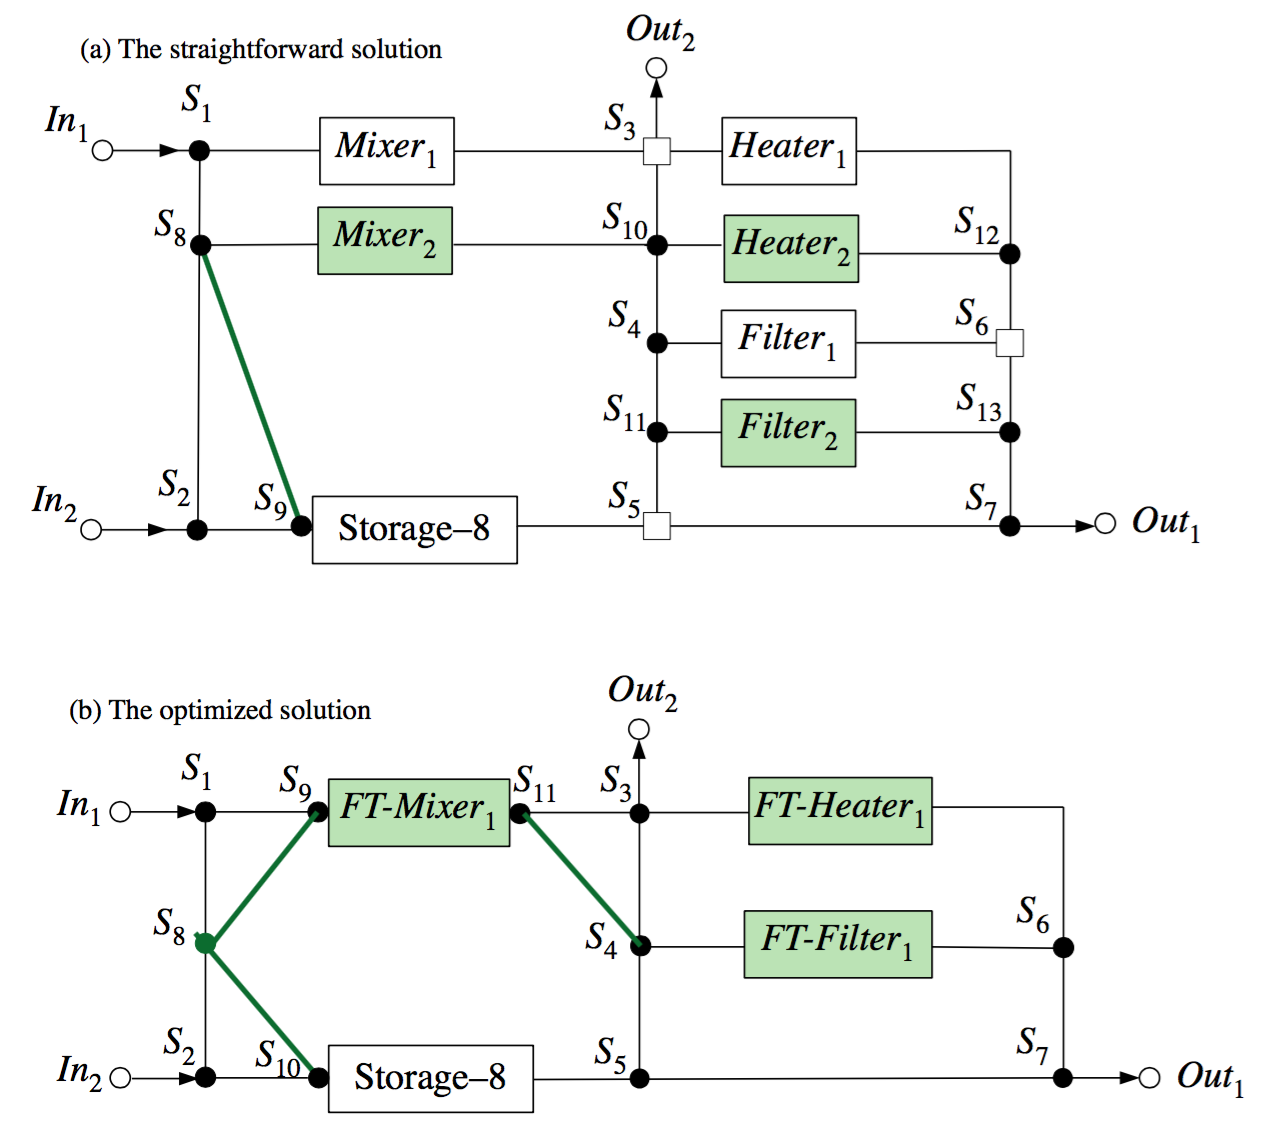
\includegraphics[scale=0.4]{figures/motivational-example-specific-fm.png}
\caption[Possible solutions for fault-tolerant architecture synthesis of the example]{Possible solutions for fault-tolerant architecture synthesis of the example}
\label{fig:motivational-solution}
\end{figure}

In the optimised solution the fault tolerant variants of filter, heater and mixer have replaced the original components. Consequently the components tolerate the faults in the fault model and are therefore able to perform their operations. Two redundant channels have been added to compensate for the two blocked channels. Routing is still possible even though there are valves failing in some switches. The cost of the architecture in \autoref{fig:motivational-solution}b is calculated to be 96. The optimised solution is therefore less costly than the straightforward solution, while at the same time tolerating all the fault scenarios possible under the given fault model. Considering the application $\mathcal{G}$ in \autoref{fig:arch-syn-application} there are four routes that will be affected by the valves failing in the switches. When the filtration and heating operation finish the resulting fluids from both operations will need to route back to the $FT$-$Mixer_1$. Consequently they need to route through $S_6$ to $S_7$ however as the valve $v_3$ is the failing valve it is still possible use the channel $S_6 \rightarrow S_7$. Recall that when the valve stuck open in the switch restricts / allows flow to the channel, we want to route to, then the fault is inconsequential. However when arriving to $S_5$ the failing valve $v_2$ in $S_5$ forces the fluid to go through Storage-8 and therefore the route is a bit longer than the optimal route. The other two routes affected are $FT$-$Mixer_1 \rightarrow FT$-$Heater_1$ and $FT$-$Mixer_1 \rightarrow Out_2$. The optimal routes would be to use the channel $FT$-$Mixer_1 \rightarrow S_3$ however as the valve $v_3$ of $S_3$ is failing it is not possible to use this channel and the desired optimal route. However the routes can use the redundant channel $FT$-$Mixer_1 \rightarrow S_4$. This allows the usage of the channel $S_4 \rightarrow S_3$ and thereby route to $FT$-$Heater_1$ and $Out_2$. It is possible now to route to any channel we want to from $S_3$ as we are routing to $S_3$ from the channel that the stuck open valve restricts / allows flow from.\\

The assumption is that the fault-tolerant architecture synthesis is part of a methodology. The steps in the methodology are as follow.

\begin{enumerate}
\item \emph{Architecture design}. An architecture $\mathcal{A}$ is designed by the designer. This architecture can be generated as an application-specific architecture, which is possible using a tool developed in \cite{wajid}.

\item \emph{Fault-tolerant architecture synthesis}. A fault-tolerant netlist is synthesised for the architecture $\mathcal{A}$ designed in the previous step while considering an application graph $\mathcal{G}$ with a deadline $d_\mathcal{G}$ and a fault model $\mathcal{Z}$.

\item \emph{Physical architecture synthesis}. A physical architecture is synthesised (generating the placements of the component) using the fault-tolerant netlist generated in step 2. The physical architecture synthesis is possible using the tool developed in \cite{michael}.

\item \emph{Fabrication}. The biochips are fabricated using the architecture $\mathcal{A}$ obtained in the previous step.

\item \emph{Testing}. All the biochips are tested to determine if they have permanent faults using techniques such as the one proposed in \cite{fault-modeling}, which is outlined in \autoref{sec:general-testing-strategy}. The exact locations of faults are determined during this step. If there are any permanent faults on the biochip not present in the fault model $\mathcal{Z}$, the biochip is discarded.

\end{enumerate}

The focus of this thesis is on the second step of the methodology: the fault-tolerant architecture synthesis problem. The thesis proposes two solutions based on metaheuristics, Simulated Annealing and Greedily Randomized Adaptive Search Procedure. The flow of the metaheuristic implementations is outlined in \autoref{fig:architecture-synthesis}. A metaheuristic explores the solution space using design transformations called moves. These are applied to the current solution in order to obtain neighbouring architecture alternatives.

\begin{figure}[H]
\centering
%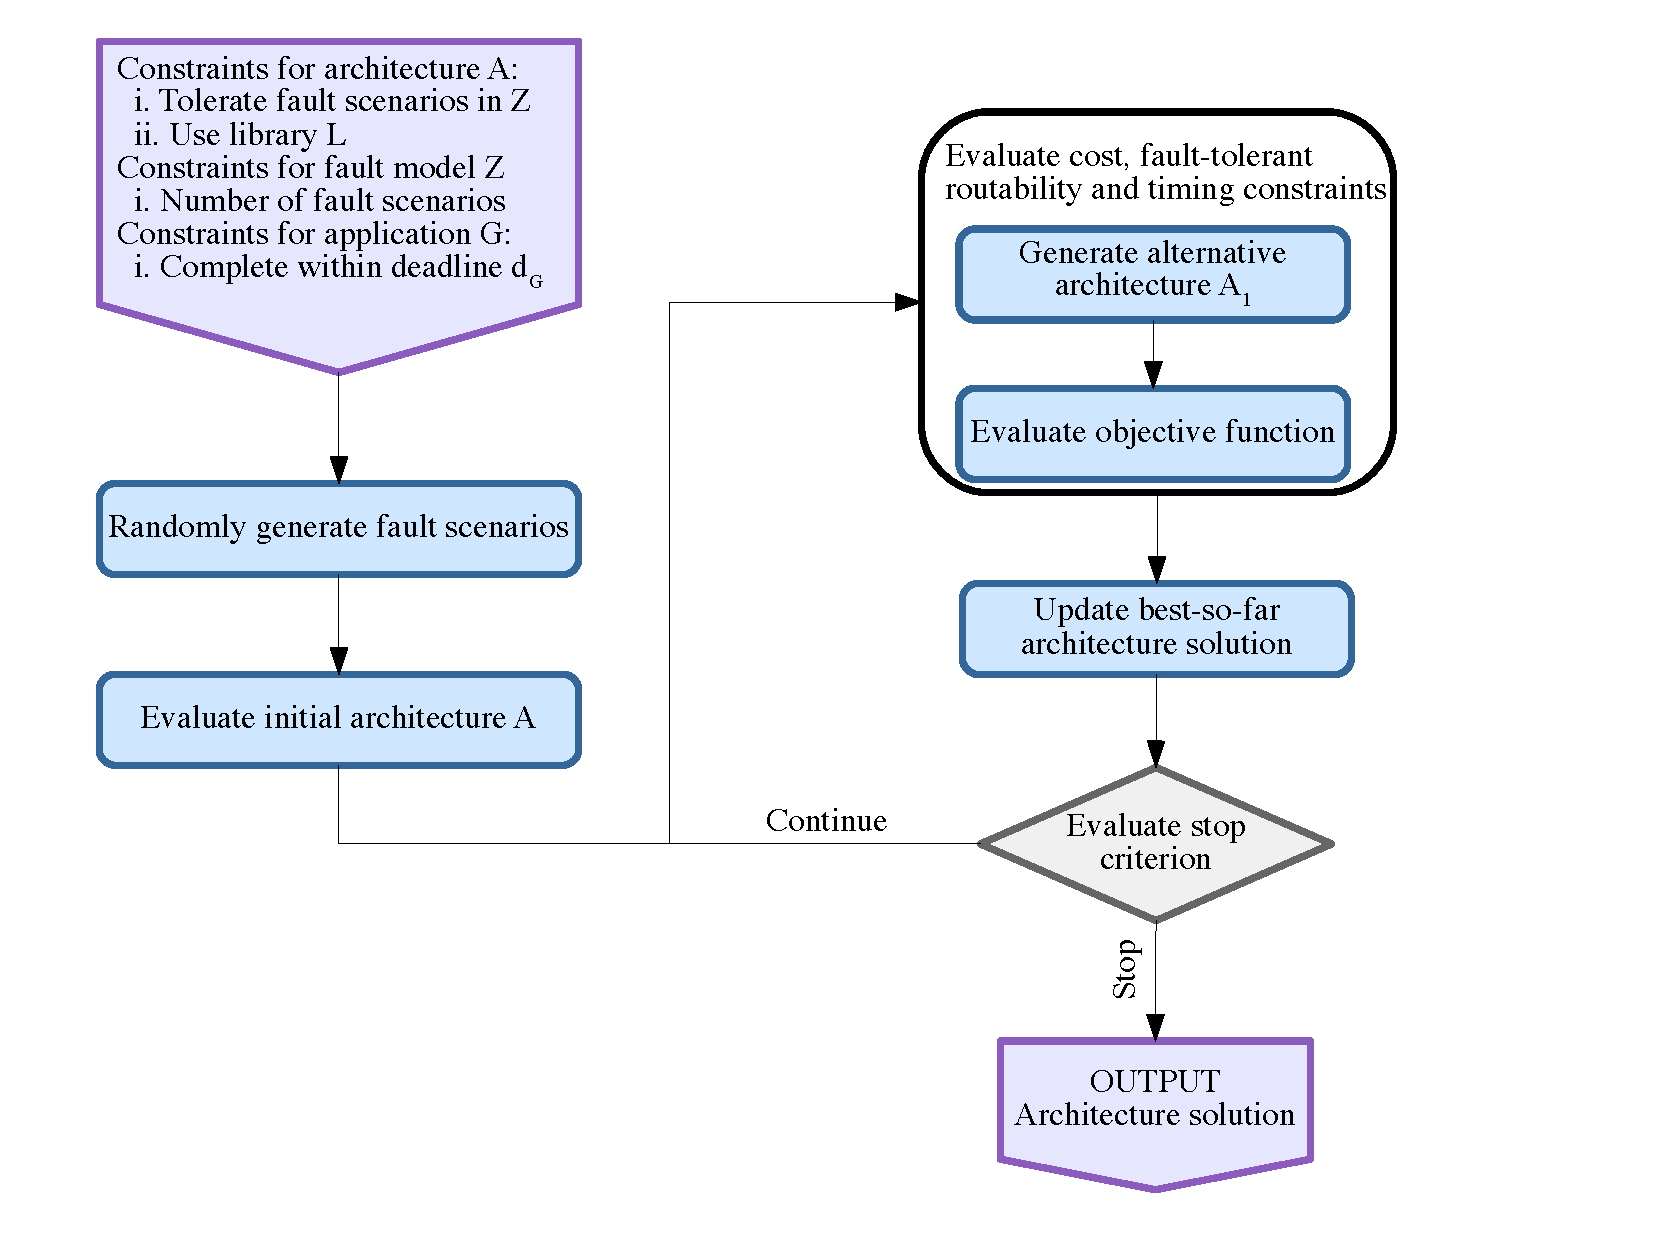
\includegraphics[scale=0.45]{figures/architecture-synthesis.pdf}
%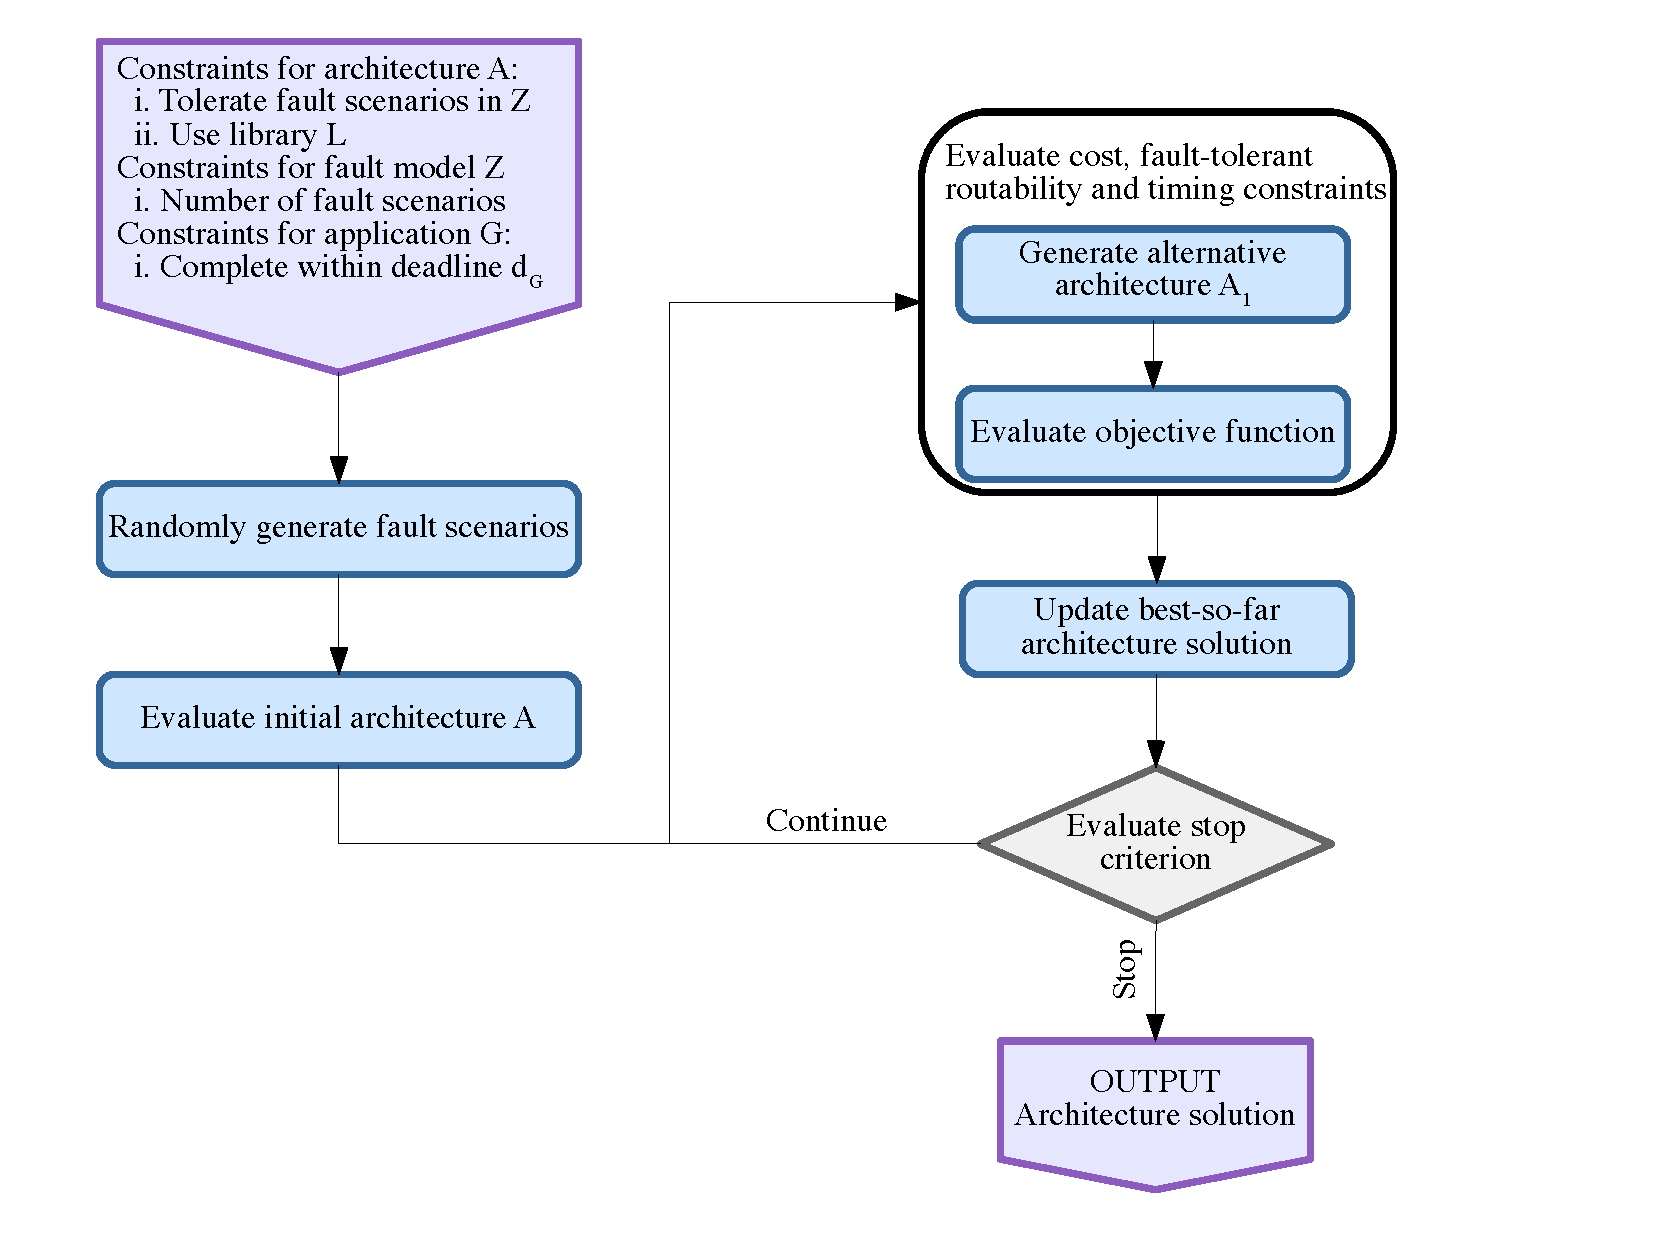
\includegraphics[width=\textwidth]{figures/architecture-synthesis.pdf}
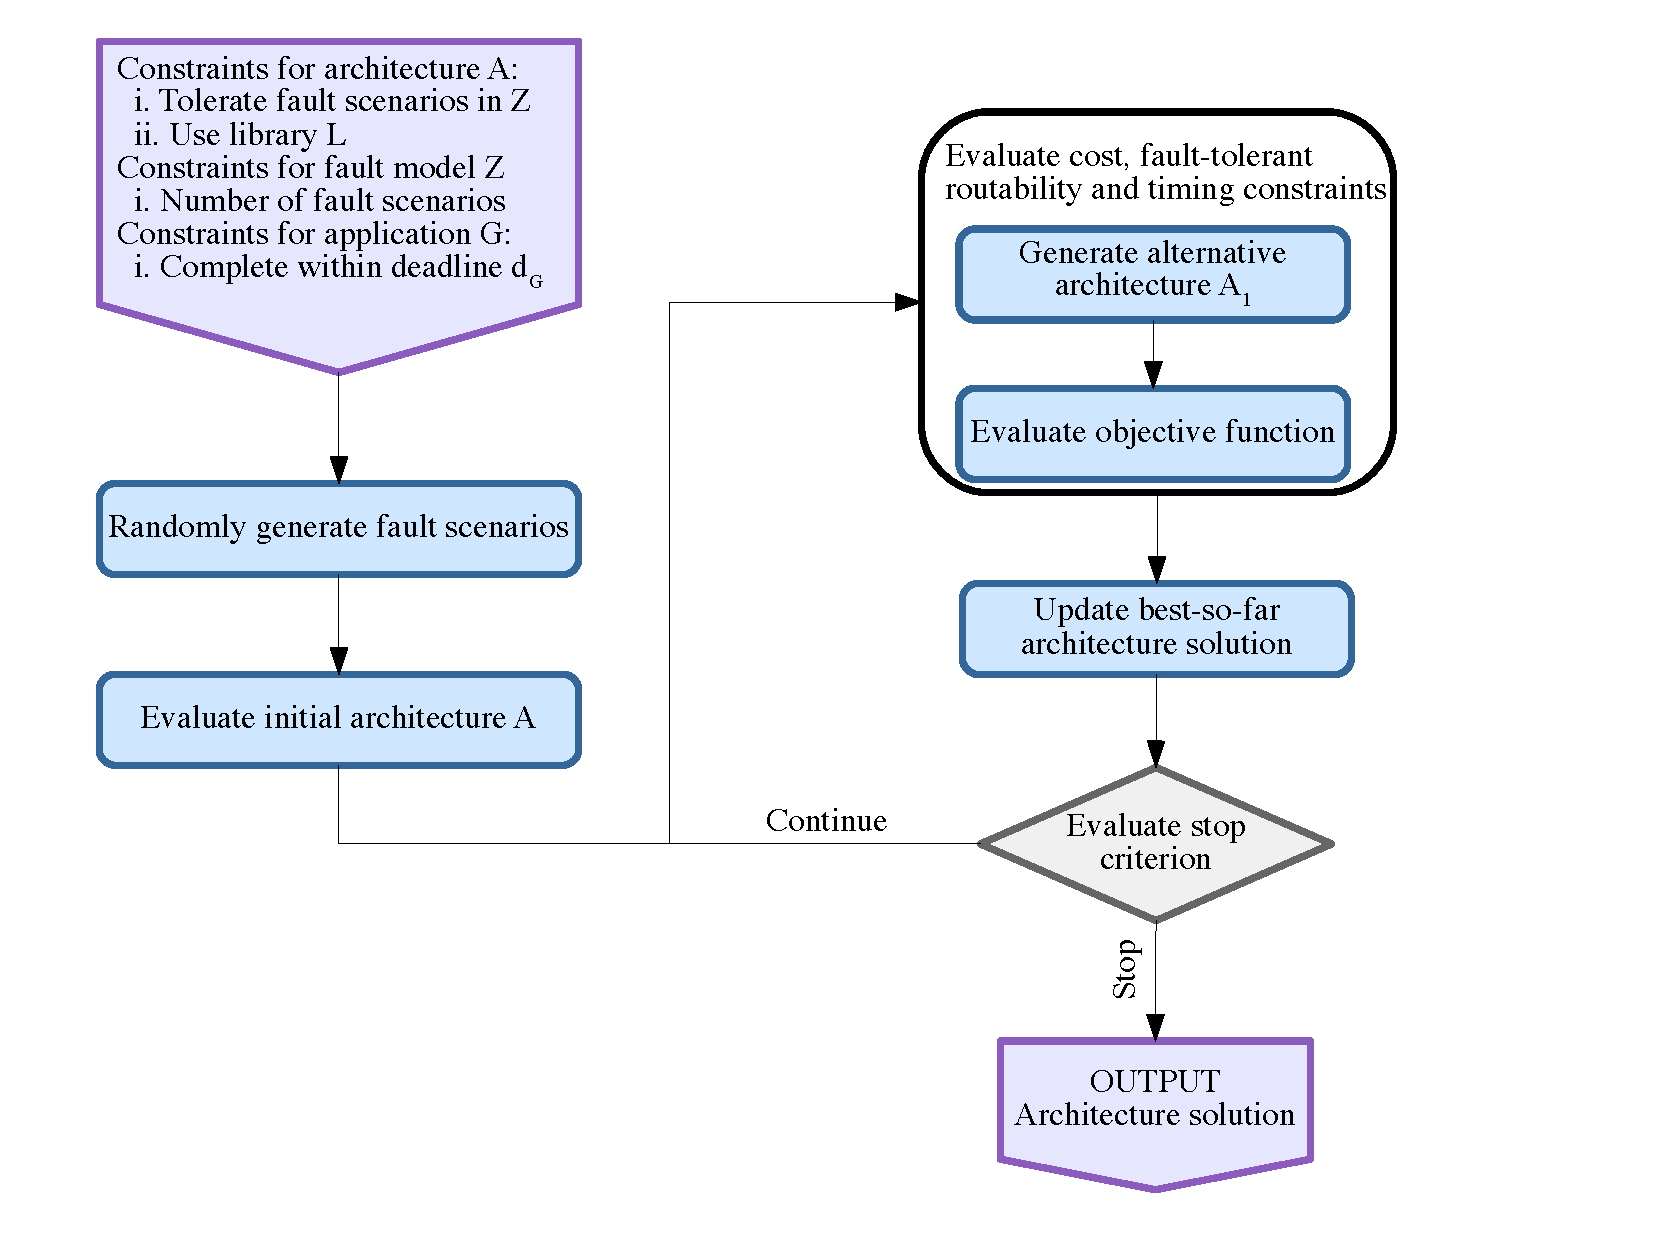
\includegraphics[scale=0.4]{figures/architecture-synthesis.pdf}
\caption[Architecture synthesis]{Architecture synthesis}
\label{fig:architecture-synthesis}
\end{figure}

One of the architecture alternatives is then selected to be the current solution. Therefore each architecture alternative is evaluated using an objective function which is described in \autoref{chap:arch-eval}. When a new architecture solution improves the objective function it is accepted and chosen as the current solution. However in some cases the Simulated Annealing metaheuristic accepts worse solution in order to escape the local minima. The metaheuristic continues to apply the moves on the determined current solution and uses the objective function to evaluate the obtained neighbouring architectures. The search terminates when a stop criterion is satisfied.\\

\section{Design Transformations}
\label{sec:moves}
In order to generate an alternative architecture a way to obtain neighbouring solutions has to be defined. This is also called \emph{moves} as mentioned. It is possible to specify multiple moves. The possible moves implemented in this thesis are as follows.
%In order to implement SA for the fault-tolerant the way to obtain a neighbouring solution has to be defined, also called \emph{moves}. The possible moves to obtain a neighbouring solution in are as follows.
\begin{enumerate}

\item \emph{Add redundant component}: In order to make a component redundant another component of that type is added to the architecture.

\item \emph{Convert regular component to the fault-tolerant version}: By virtue of the component library $\mathcal{L}$ given in \autoref{tab:component-library} with fault-tolerant components a component can be changed to its fault-tolerant version provided it is a component with a fault-tolerant version.

\item \emph{Add connection between two components}: A redundant connection is added between the two components.

\item \emph{Remove redundant component}: A redundant component is removed from the architecture. Note that it is only a redundant component that can be removed, i.e. none of the original components in the architecture are removed.

\item \emph{Convert fault-tolerant component to the regular version}: This move is the reverse of move 2 as no component is fault-tolerant in the initial architecture.

\item \emph{Remove connection}: A redundant connection is removed from the architecture. Note that it is only a redundant connection that can be removed. None of the original connections in the architecture are removed.

\end{enumerate}

Let us consider the architecture from \autoref{fig:moves}a as the current solution $\mathcal{A}^{current}$. By applying the following moves: add redundant connection between $S_4$ and $Heater_1$, convert $Mixer_1$ to its fault-tolerant version and add redundant component $Filter_2$, we obtain the neighbouring architectures from \autoref{fig:moves}b, c and d respectively.

\begin{figure}[H]
\centering
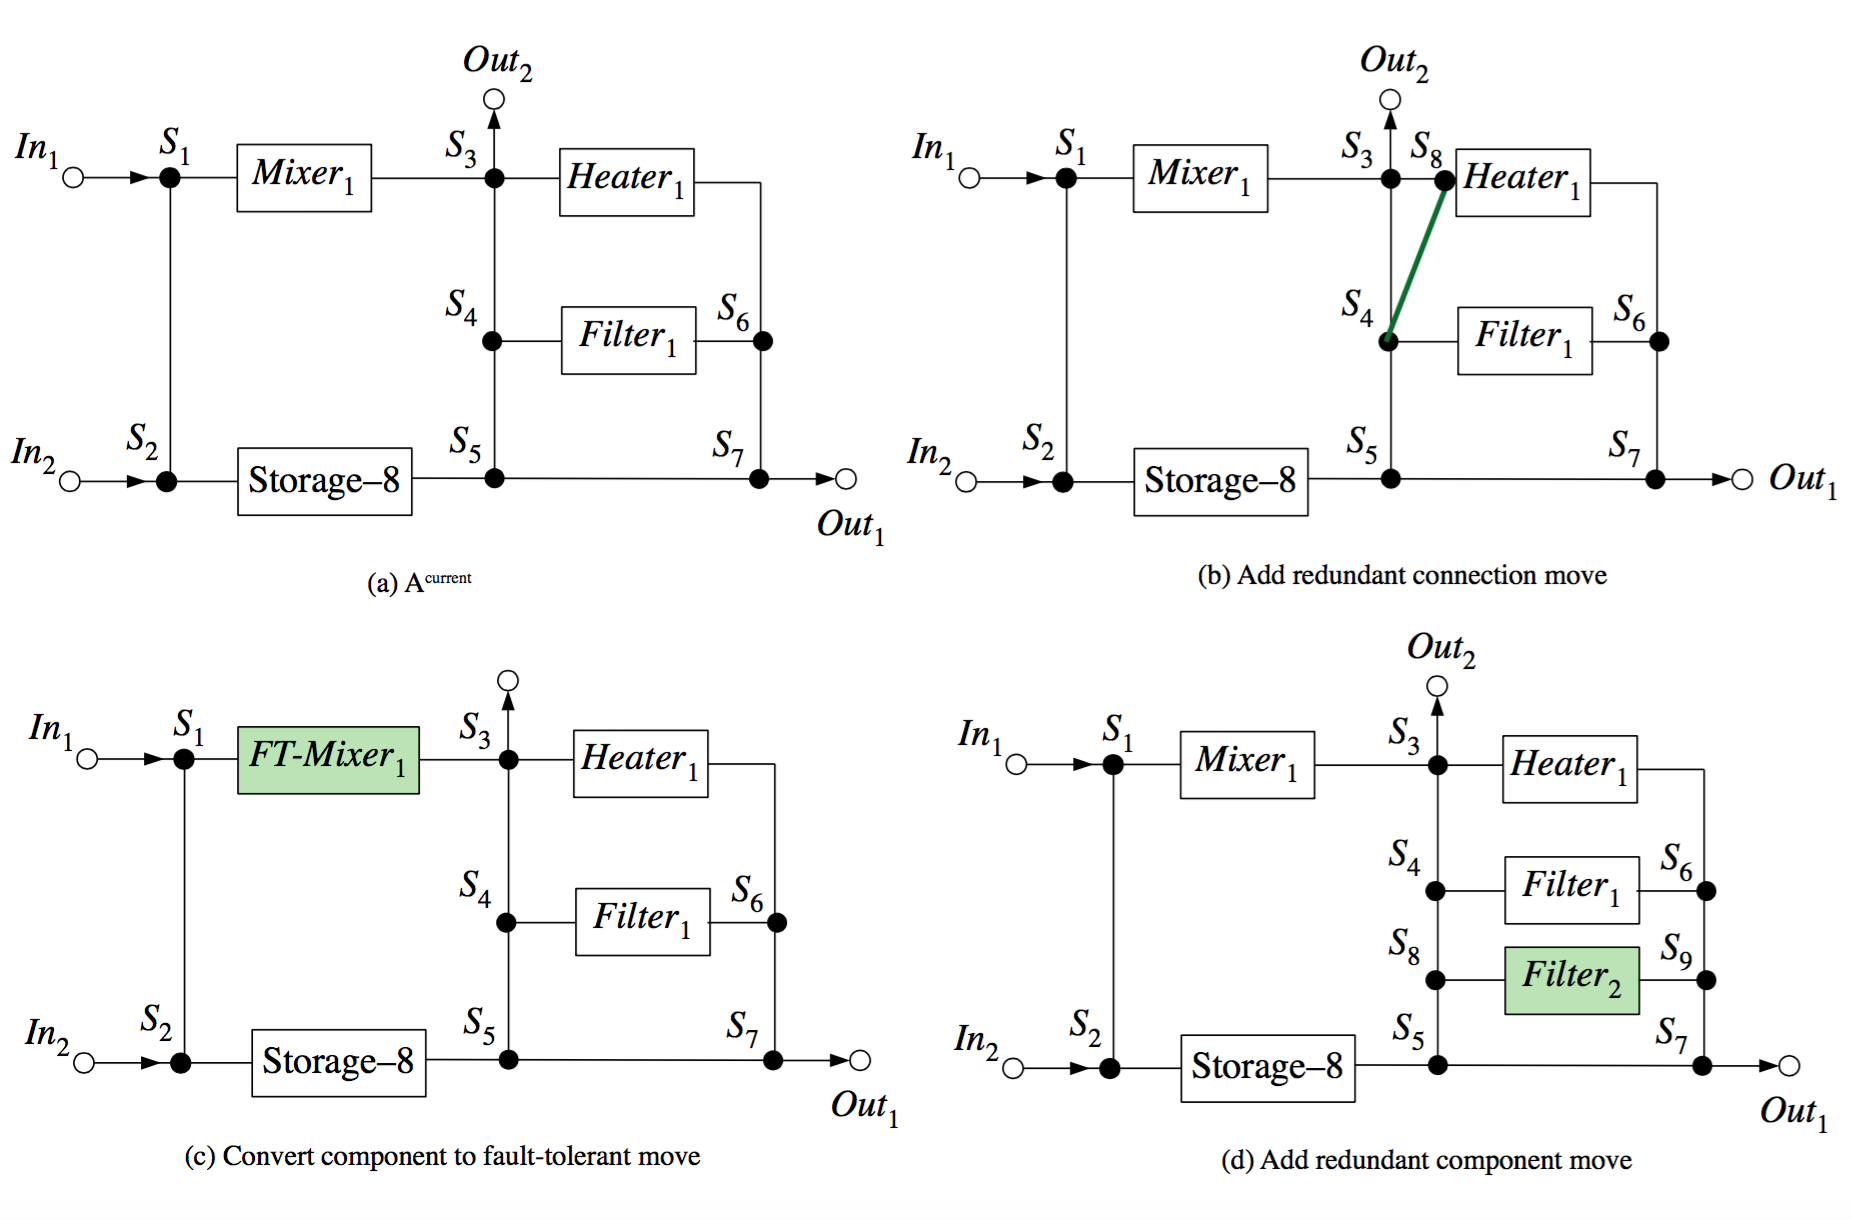
\includegraphics[scale=0.35]{figures/moves.png}
\caption[Example of neighbouring solutions]{Example of neighbouring solutions}
\label{fig:moves}
\end{figure}

%Therefore in this thesis two solutions are proposed to the fault-tolerant architecture synthesis problem. The two solutions will be described in the following sections.


\section{Simulated Annealing Architecture Synthesis}
\label{sec:sa}
As a solution to the fault-tolerant architecture synthesis problem we propose a Simulated Annealing approach. Simulated Annealing, henceforth \emph{SA}, is a metaheuristic whose inspiration originates from a technique in metallurgy. In metallurgy, annealing is the process used to temper or harden metals and glass by heating them to a high temperature and then gradually cooling them, thus allowing the material to reach a low-energy crystalline state \cite{arti-intel}. In the following sections the concept of SA will be explained and how it is implemented for the fault-tolerant architecture synthesis problem.

\subsection{Concept}
The idea of SA is to randomly create an initial solution, $s_0$, and choose an initial temperature, $t_0$. A neighbouring solution of $s_0$ is explored to see if that solution is an improvement. The quality of the solutions is determined by a \emph{cost function}. If the neighbouring solution improves the current solution, that solution is chosen as the current one and the temperature is reduced according to a \emph{cooling schedule}. However if the neighbouring solution is worse it is accepted with a certain probability. If the algorithm only accepted a solution determined to be an improvement it would converge towards the local optimum and not the global optimum.

The idea is that when the temperature is high a large part of the solution space is explored. Accordingly at high temperatures almost any solution is accepted regardless of the quality. As the temperature decreases the simulation gradually becomes more and more reluctant to accept inferior solutions. When the temperature becomes low enough SA will only accept solutions that improves the current solution. This causes it to become stable at a local optimum. If the cooling is slow then the local optimum is a good approximation on the global optimum. The probability, $p(s)$, that an inferior solution, $s$, will be chosen is given by the exponential expression.
$$p(s) = e^{-\delta / t}$$
where $\delta$ is the cost increase from the previous solution, and $t$ is the temperature. The probability is inspired by the laws of thermodynamics.

\subsection{Implementation}
SA takes as input the initial architecture $\mathcal{A}$, the component library $\mathcal{L}$, the application graph $\mathcal{G}$, and a fault model $\mathcal{Z}$ and produces a fault-tolerant netlist of minimum cost. For the evaluation of each architecture alternative the SA-based architecture synthesis uses the cost function described in \autoref{chap:arch-eval}. By the fact that SA receives the initial architecture $\mathcal{A}$ as an input there is no need to randomly generate an initial solution. The algorithm is shown in \autoref{alg:sa}.

\begin{figure}[H]
\centering
\begin{algorithmic}[1]
\Function{SimulatedAnnealing}{$\mathcal{A}, \mathcal{L}, \, \mathcal{G}, \mathcal{Z}$}
	\State $t \gets t_0$\Comment{Temperature is initialized, $t_0 > 0$}
      \While{$t \leq t_{termination}$}
	\For {$i \gets 0$ to $iterations$}
		\State $\mathcal{A}' \gets \Call{RandomNeighbor}{\mathcal{A}}$
		\If{$\Call{Cost}{\mathcal{A}'} < \Call{Cost}{\mathcal{A}} \vee \Call{Random}{0, 1} < e^{-\delta / t}$}
		\State $\mathcal{A} \gets \mathcal{A}'$ 
		\EndIf
	\EndFor
	\State $t \gets \Call{ReduceTemperature}{t}$\Comment{Temperature is reduced}
      \EndWhile
	\State \textbf{return} $\mathcal{A}$
    \EndFunction
\end{algorithmic}
\caption[Implementation of Simulated Annealing]{Implementation of Simulated Annealing}
\label{alg:sa}
\end{figure}

Deciding whether or not to accept the architecture $\mathcal{A}'$ or keep the current one $\mathcal{A}$ is done in line 6. A superior architecture is always accepted ($\delta < 0$) but an inferior solution is accepted with the probability $p(s) = e^{-\delta / t}$. The criterion is met by generating a number uniformly at random between 0 and 1, which must be less than the acceptance probability, $p(s)$.

The SA-based synthesis generates new architecture alternatives by performing moves on the current solution which is line 5 of the algorithm. The moves are described in detail in \autoref{sec:moves}. The moves are chosen uniformly at random. Each move is randomised in itself. Adding a connection picks two components uniformly at random and adds a connection between them. Similarly converting a component to its fault-tolerant version move choses the component uniformly at random, provided it has a fault-tolerant version. This randomness applies to each move done by SA to obtain a neighbouring architecture.

The temperate cooling schedule consists of four parameters: initial value, reduction function, termination value and number of iterations at each temperature. The initial value should be high such that initially the acceptance rate is close to 100\%. This ensures that the entire solution space is explored. The reduction function determines the speed of the temperature cooling. The implementation of SA uses this reduction function.
$$\Call{ReduceTemperature}{t} = k \times t$$
where $k < 1$. In order to ensure the cooling down is slow a value of $0.999$ has been used for $k$.\\
Performing many iterations at each temperature ensures a more thorough exploration of the solution space. Considering that superior solutions are accepted unconditionally spending more time at each temperature has a tendency to lead to better final solutions. The number of iterations at each temperature, $iterations$, can be used to scale the running time of the algorithm to ensure more exploring of the solution space. A value of 1 has been used to obtain results. Experimenting more with the number of iterations is a possible optimisation.\\
The cooling should continue until the temperature is zero. A value of 0.1 for the termination temperature has provided good results in this thesis. However often the heuristic settles for a non-improving stable solution long before the temperature reaches zero. There could also be experimented more with the termination temperature.

\begin{figure}[H]
\centering
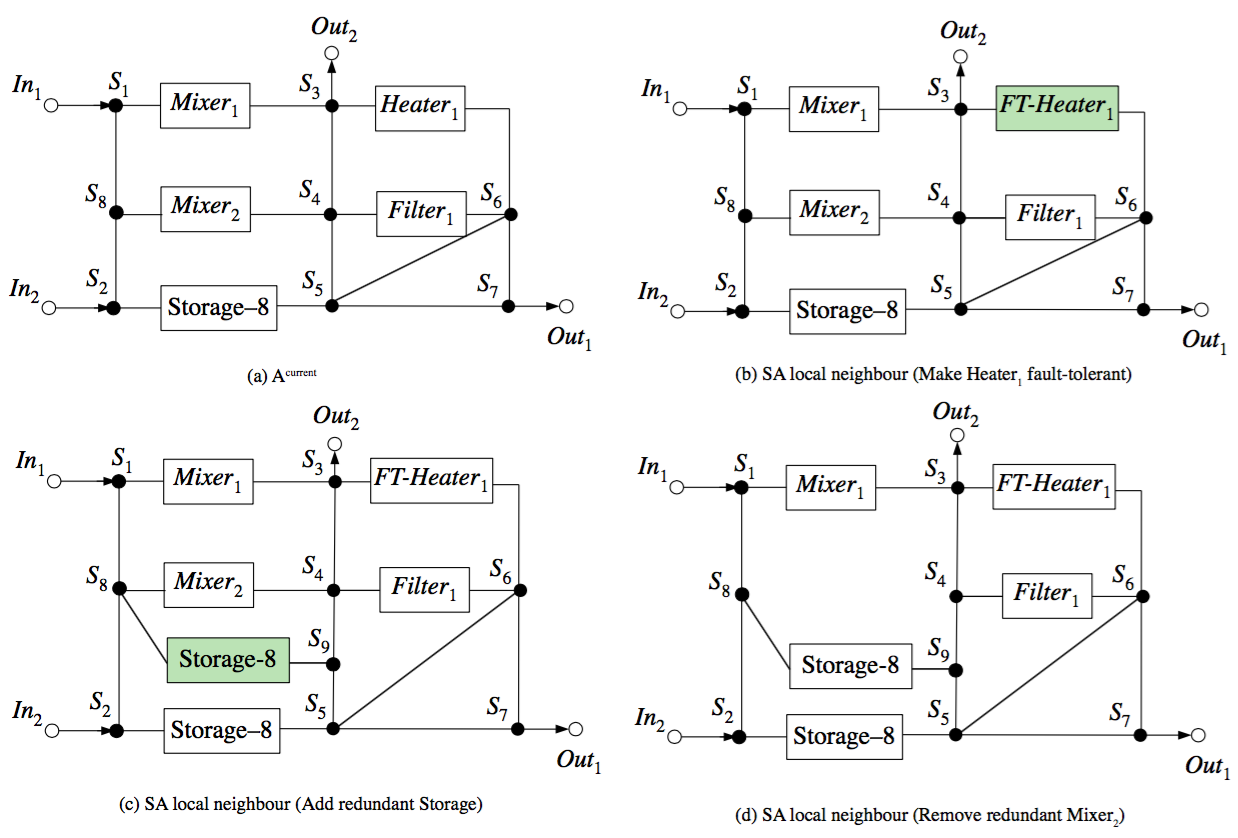
\includegraphics[width=\textwidth]{figures/SA-example.png}
\caption[Simulated Annealing example]{Simulated Annealing example}
\label{fig:sa-example}
\end{figure}

Let us consider the example in \autoref{sec:prob-for} with the initial architecture given in \autoref{fig:arch-syn-arch}, the application in \autoref{fig:arch-syn-application} and the faults in \autoref{tab:arch-valve-faults} and \autoref{tab:arch-channel-faults} to illustrate how SA works. \autoref{fig:sa-example}a is the current solution, $\mathcal{A}^{current}$, where a number of moves have been applied to the initial architecture in order to obtain $\mathcal{A}^{current}$. From here we can apply most of the moves described in \autoref{sec:moves}. Uniformly at random we pick a move, which gives us the architecture alternative \autoref{fig:sa-example}b. This move is accepted since it now tolerates the channel fault of $Heater_1$, which means it improves the current solution and is thereby chosen as the current solution, $\mathcal{A}^{current}$. From this solution we apply a random move again to obtain the architecture in \autoref{fig:sa-example}c, which is adding a redundant storage component. This move is accepted and chosen as $\mathcal{A}^{current}$ although it does not improve the current solution. It only adds more valves and connections without contributing to the completion of the application. The move is accepted due to the randomness of SA when deciding whether to accept inferior solutions. As in the previous steps we pick a random move to see how it affects the current solution. This move chosen is removing the redundant component, $Mixer_2$. However this move is not accepted by SA as $Mixer_1$ is affected by a fault such that is unable to perform mixing, and by virtue of removing $Mixer_2$ the architecture cannot perform mixing. Therefore this move is not accepted even though SA randomly accepts inferior solutions. This continues until SA reaches its termination temperature.

\section{GRASP Architecture Synthesis}
\label{sec:grasp}
Greedily Randomized Adaptive Search Procedure, henceforth \emph{GRASP}, is a metaheuristic for combinatorial optimisation \cite{grasp}. Combinatorial optimisation is a problem that consists of finding an optimal object from a finite set of objects.

\subsection{Concept}
GRASP is an iterative metaheuristic. Each iteration consists of two phases: a construction phase and a local search phase. In the construction phase the GRASP algorithm builds a solution based on a list of candidate design transformations. The local search phase explores the neighborhood of the built solution to find the local optimum. GRASP runs for a number of iterations and returns the best solution found, i.e. the found solution that minimises the cost function the most.\\
In a greedy algorithm a solution is constructed one element at a time. At each step in the construction a set $C$ of candidate elements that can be added to the solutions at that step is constructed. A greedy function is applied to each element in $C$ and the elements are ranked according to their greedy function values. A best ranked element is added to the solution. By virtue of this the set $C$ is updated and the greedy function changes. The process continues until $C = \emptyset$. By randomly generating initial solutions a multi-start procedure will eventually find the global optimum. Using greedy solutions as starting points for local search however in a multi-start method will generally lead to good although often suboptimal solutions due to the small amount of variability in greedy solutions and the small likeliness that a greedy starting solution is in the vicinity of the global optimum \cite{grasp}. A \emph{semi-greedy} heuristic adds variability to the greedy algorithm. The candidate elements are ranked according to their greedy function values. Afterwards the well ranked candidates are placed in a \emph{restrictive candidate list} (RCL) and an element from RCL is selected at random and added to the solution. There are two schemes to build an RCL \cite{grasp}:
\begin{enumerate}
\item In the \emph{cardinality} based scheme an integer $k$ is fixed and the $k$ top ranked elements are placed in the RCL

\item In the \emph{value} based scheme all candidate elements with greedy function values within $a$\% of greedy value are placed in the RCL, where $a \in [0, 100]$

\end{enumerate}

The GRASP algorithm therefore builds initial solutions by applying design transformations on elements from the RCL.

\subsection{Implementation}
The implementation of GRASP in this thesis is inspired by the implementation given in \cite{domi-grasp} and adapted to the fault-tolerant architecture synthesis problem. The implementation is shown in \autoref{alg:grasp}. GRASP takes as input the initial architecture $\mathcal{A}$, the component library $\mathcal{L}$ and a fault model $\mathcal{Z}$. Additional parameters to the algorithm are the number of iterations, $NoI$, for GRASP to run, the size of the candidate list $cl$, the number of unsuccessful iterations, $ui$, after which the algorithm increases the size of $cl$ with $cli$. Similarly there is a parameter specifying the number of iterations, $NbI$, for the local search.

\begin{figure}
\centering
\begin{algorithmic}[1]
\Function{GRASP}{$\mathcal{A}, \mathcal{L}, \, \mathcal{G}, \mathcal{Z}, NoI, cl, ui, cli, NbI$}
	\State $\mathcal{A}^{best} \gets \mathcal{A}$
	\State $Cost^{best} \gets \Call{Cost}{\mathcal{A}}$
	\State $\#ui \gets 0$
      \While{$i < NoI$}
	\State $CL \gets \Call{CreateCandidates}{\mathcal{A}, cl}$\Comment{Phase 1}
	\State $RCL \gets \Call{ChooseCandidates}{CL}$
	\State $\mathcal{A}' \gets \Call{ApplyDesignTransformations}{\mathcal{A}, RCL}$
	\State $\mathcal{A'} \gets \Call{HillClimbing}{\mathcal{A}', NbI}$\Comment{Phase 2}
		\If{$\Call{Cost}{\mathcal{A}'} < Cost^{best}$}
			\State $\mathcal{A}^{best} \gets \mathcal{A}'$ 
			\State $Cost^{best} \gets \Call{Cost}{\mathcal{A}^{best}}$
			\State $\#ui \gets 0$
		\Else
			\State $\#ui \gets \#ui + 1$
		\EndIf
		\If{$\#ui \geq ui$}
			\State $cl \gets cl \times cli$
			\State $\#ui \gets 0$
		\EndIf
		\State $i \gets i + 1$
      \EndWhile
	\State \textbf{return} $\mathcal{A}^{best}$
    \EndFunction
\Function{HillClimbing}{$\mathcal{A}, iterations$}
	\State $j \gets 0$
	\While{$j < iterations$}
		\State $\mathcal{A}' = \Call{RandomNeighbor}{\mathcal{A}}$
		\If{$\Call{Cost}{\mathcal{A}'} < \Call{Cost}{\mathcal{A}}$}
		 	\State $\mathcal{A} \gets \mathcal{A}'$
		\EndIf
		\State $j \gets j + 1$
	\EndWhile
	\State \textbf{return} $\mathcal{A}$
\EndFunction
\end{algorithmic}
\caption[Implementation of GRASP]{Implementation of GRASP}
\label{alg:grasp}
\end{figure}

The algorithm initializes the cost of the best known solution to the cost of the initial architecture. Furthermore the number of unsuccessful iterations $\#ui$ is initialized as 0 where an unsuccessful iteration is defined as not improving the best known solution. GRASP performs two phases: solution construction and local search. During the construction phase GRASP creates the candidate list $CL$ of $cl$ potential candidate components that will be transformed. The selection of potential candidates is done by ranking each component $M \in N$ of $\mathcal{A}$ by the number of fault scenarios affecting the component. A fault scenario is affecting a component if it contains a valve fault or channel fault affecting the component or if it contains a channel fault that blocks an input or output channel of the component. Only $cl$ components with the highest ranking are selected by GRASP. However the number $cl$ of potential candidate components does not remain constant throughout the search. If $ui$ number of iterations has passed since improving the best known solution $\mathcal{A}^{best}$ the size $cl$ of the potential candidate list is increased by $cli$ (lines 17-20).\\
From the candidates list $CL$ GRASP selects a random subset $RCL$ of candidates (line 7). The size of the subset is chosen uniformly at random ranging from one candidate to the full set of potential candidates. Each component from the restricted candidate list RCL is then randomly applied to one of five design transformations (line 8 in the algorithm):
\begin{enumerate}
\item Add a redundant component to the architecture to compensate for the component

\item Convert the component to its fault-tolerant version

\item Convert the component to its fault-tolerant version and add a redundant incoming connection to the component

\item Convert the component to its fault-tolerant version and add a redundant outgoing connection from the component

\item Convert the component to its fault-tolerant version and add redundant connections for the component both incoming and outgoing

\end{enumerate}

In the second phase GRASP performs local search (line 9). In this GRASP implementation a simple Hill Climbing, henceforth \emph{HC}, algorithm is used. The HC algorithm generates new architecture alternatives by performing moves on the current solution (line 28). The possible moves are described in \autoref{sec:moves}. The moves are chosen uniformly at random. Similarly to SA the moves are also randomized in itself, e.g. it will pick two random components to connect when adding a connection. It then evaluates the architecture alternative and if it is deemed less costly it is chosen as the new solution in HC (line 29-31). When the local search finishes it will return the best solution found. If the solution found by HC is better than the best known solution in GRASP the new solution is chosen as the best solution and $\#ui$ is reset to 0 as it has been a successful iteration. If it is deemed more costly than the best known solution then it is an unsuccessful iteration and $\#ui$ is incremented by 1 (line 10-16). The GRASP algorithm returns the best found solution $\mathcal{A}^{best}$ in terms of the objective function defined in \autoref{chap:arch-eval}.

The GRASP algorithm consists of many defined parameters. The number of iterations of the algorithm, size of the candidate list, number of unsuccessful iterations after which the algorithm increases the size of the candidate list with a certain amount. Lastly the number of iterations in the local search also has to be defined. In this thesis the number of iterations of GRASP has been 50 which has provided good results. The initial size of the candidate list has been 2 where it has been increased by a factor of 2 each time the maximum number of unsuccessful iterations has been reached. The number of unsuccessful iterations has been ranging from 5 to 10 where both have provided good results. The number of iterations in the local search phase has ranged between 50 and 100 where good results have been produced within this range.

\begin{figure}
\centering
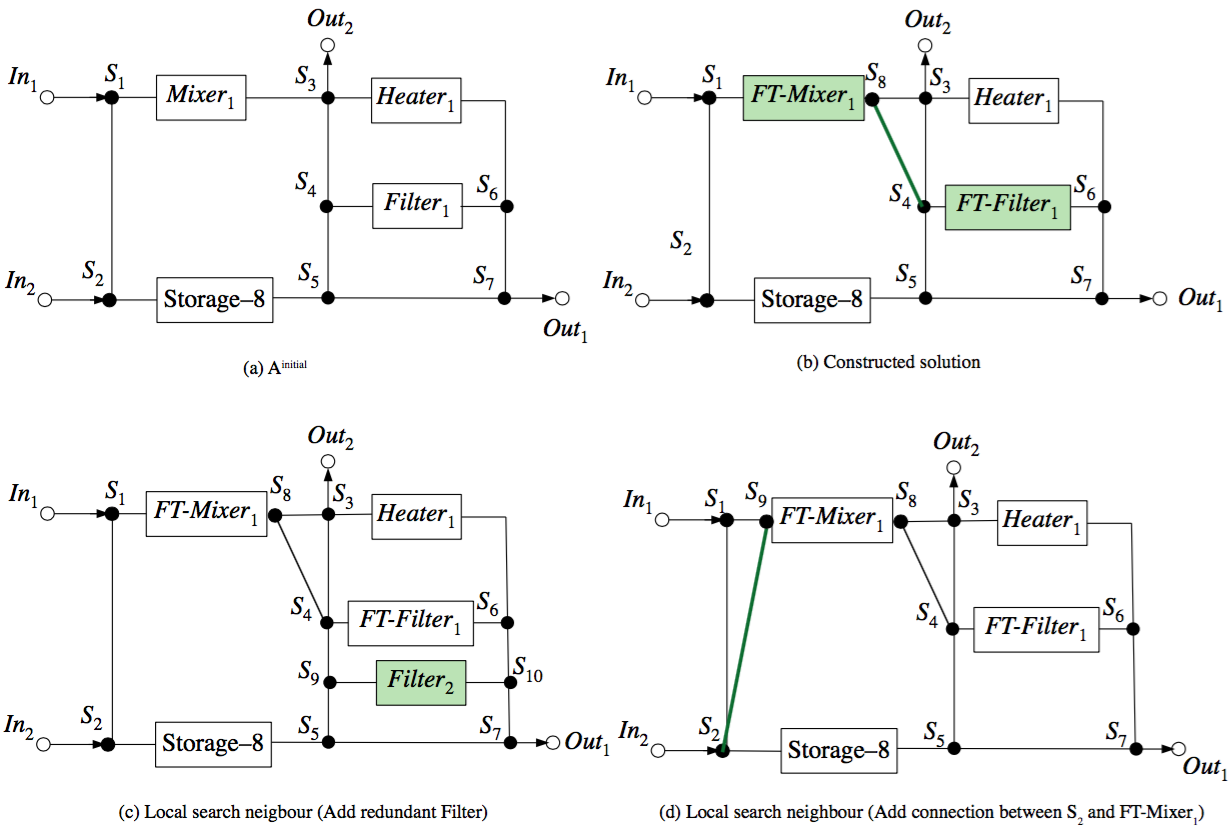
\includegraphics[width=\textwidth]{figures/GRASP-example.png}
\caption[Greedily Randomized Adaptive Search Procedure example]{Greedily Randomized Adaptive Search Procedure example}
\label{fig:grasp-example}
\end{figure}

Let us consider the example in \autoref{sec:prob-for} with the initial architecture given in \autoref{fig:arch-syn-arch}, the application in \autoref{fig:arch-syn-application} and the faults in \autoref{tab:arch-valve-faults} and \autoref{tab:arch-channel-faults} to illustrate how GRASP works. Each iteration of GRASP starts with the initial architecture, $\mathcal{A}^{initial}$, shown in \autoref{fig:grasp-example}a. The candidate list has well ranked components, where the ranking is decided by the fault scenarios affecting the component. Therefore $Mixer_1$, $Heater_1$ and $Filter_1$ are in this candidate list. Randomly a subset of this candidate list is chosen and each is randomly applied to one of the five moves described earlier. $Mixer_1$ is converted to its fault-tolerant version and has an added outgoing connection and $Filter_1$ is converted to its fault-tolerant version. This gives us the constructed solution shown in \autoref{fig:grasp-example}b, which is the first phase of GRASP. Then the local search starts from \autoref{fig:grasp-example}b to obtain the local optimum, i.e. it only accepts improving solutions. At random the local search picks a move from the possible moves described in \autoref{sec:moves}. It adds a redundant $Filter_2$ to the architecture, which provides the architecture in \autoref{fig:grasp-example}c. This architecture is however not accepted as it adds more valves and connections without contributing to the completion of the application. $FT$-$Filter_1$ can perform the filtering and therefore the redundant $Filter_2$ is not needed. Therefore \autoref{fig:grasp-example}b is still the current solution and it applies another a random move, which is adding a connection between $S_2$ and $FT$-$Mixer_1$. This move contributes to the completion of the application as it was not possible to route from $In_1$ or $In_2$ to $FT$-$Mixer_1$ due to blocked channels. The local search continues until the maximum number of iterations in the local search has been reached. When the local search finishes GRASP will update the best known solution if, and only if, the solution found by local search is deemed better than the best known. Afterwards GRASP restarts from the initial architecture, $\mathcal{A}^{initial}$.

\section{Summary}
This chapter specifies that the problem addressed in this thesis is obtaining a fault-tolerant netlist given an initial architecture, a component library, an application graph, and a fault model. The general flow of the architecture synthesis is described which consists of generating an architecture alternative by performing a design transformation where six possible design transformations have been defined. The chapter proposes two solutions to the fault-tolerant architecture synthesis problem, Simulated Annealing and Greedily Randomized Adaptive Search Procedure. These two algorithms are metaheuristics that have been adapted to this problem. Both proposed solutions rely on randomisation to obtain architecture alternatives.